\documentclass[a4paper, draft]{ecustthss}
\def\thetitle{一种用于脑机接口的探测P300的Boosting算法}
\def\class{电自091}
\def\studentnumber{10093409}
\def\myname{王翔}
\def\translation{(文献翻译)}
\title{\thetitle}
\def\eabstract{abstract}
\def\ekeywords{keywords}

\usepackage[chinese]{babel}

\begin{document}
  \pagestyle{translation}
  \begin{eabstract}
	This paper describes the the functions provided by
	the \emph{pkuthss} document template,
	and provides itself as an example to illustrate
	the usage of the document class.
  \end{eabstract}
  \begin{figure}
    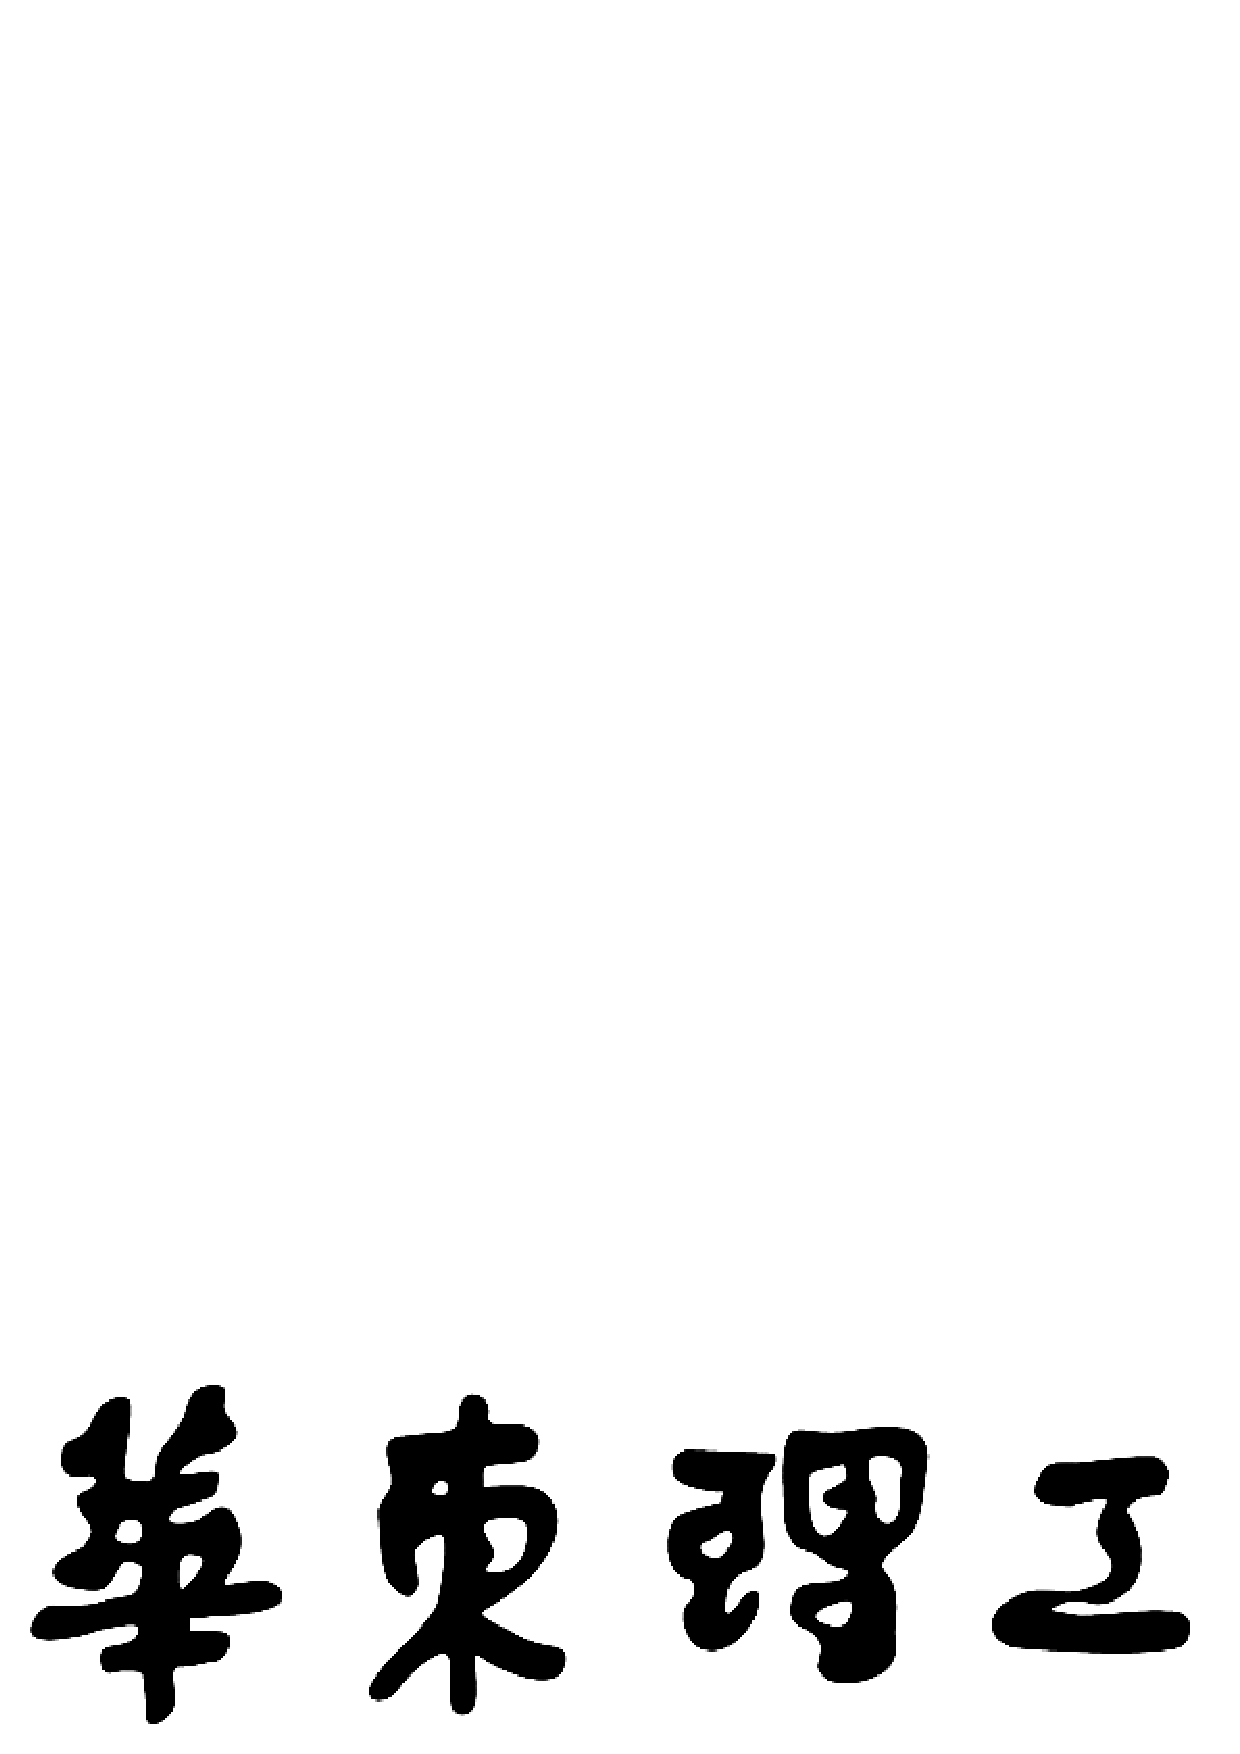
\includegraphics[height=1in]{img/ecust_words_logo}
    \caption{华东理工大学校徽}
    \label{words_logo}
  \end{figure}
  \section{\thetitle}
\end{document}
